% -*- coding: GBK2312 -*-

%\chapter{绪论} \label{chpt:A}

\chapter{绪论}

%来自wikipedia
按照机器学习以及认知科学领域普遍认同的定义,人工神经网络是一种可以根据外部信息进行自适应的仿生数学模型.如今在计算机相关技术中,人工神经网络是如今在计算机识别和控制、统计规划、医学以及生物研究领域,乃至社会经济等领域都具有广泛应用价值的研究方向.

\section{人工神经网络与人类神经活动研究}

%以下内容来自
%https://blog.csdn.net/jinking01/article/details/103344186?spm=1001.2101.3001.6650.5&utm_medium=distribute.pc_relevant.none-task-blog-2%7Edefault%7EBlogCommendFromBaidu%7ERate-5.pc_relevant_paycolumn_v3&depth_1-utm_source=distribute.pc_relevant.none-task-blog-2%7Edefault%7EBlogCommendFromBaidu%7ERate-5.pc_relevant_paycolumn_v3&utm_relevant_index=8

人工神经网络技术领域具有很深刻的多学科领域交叉的历史背景,这可以追溯到医学和生物研究领域对人类神经活动的研究模拟. 根据奥地利医生 Franz Joseph Gall 对人类神经活动依赖于人体脑部的功能的论断, 人类对神经活动的研究进入正轨. 而意大利细胞学家 Camillo Golgi 发明的 Golgi染色法 通过对脑组织切片进行染色并观测其微观结构, 确立了对人体神经网络的微观研究方式.西班牙神经组织学家 Santiago Ramón y Cajal 在此基础上进一步改进染色技术,并通过大量实验确认了神经细胞中神经元功能和结构的独立性.

1943年,基于 Golgi 和 Cajal 对生物神经系统运行原理的一系列深入研究, Warren McCulloch 和 Walter Pitts 首次提出借鉴已知神经细胞运行机制的数学模型 M-P 模型. M-P 模型作为最简的人工神经网络的架构, 开辟了人工神经网络研究这个新的计算机科学领域.

\section{人工神经网络发展}
\begin{figure}
	\centering
	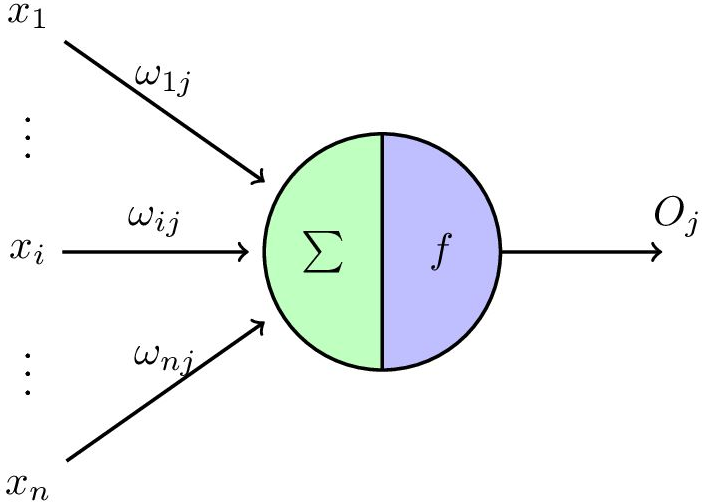
\includegraphics[scale=0.7]{Figures/mpmodel.png}
	\caption{M-P 模型}
\end{figure}
\begin{figure}
	\centering
	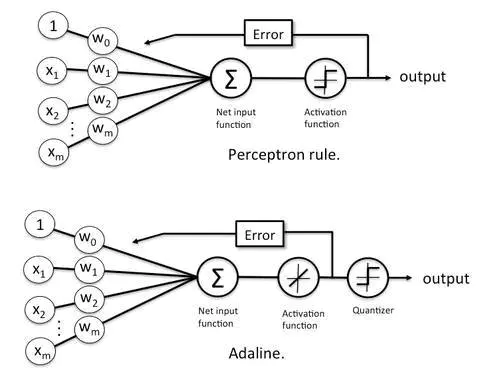
\includegraphics[scale=0.7]{Figures/perceptron.png}
	\caption{Perceptron 模型以及其改进模型 Adaline 网络}
\end{figure}

M-P模型的提出证明仿神经网络的数学模型在一定程度上可以实现逻辑和算术函数的功能.而20世纪40年代末的 Donald Olding Hebb 通过在数学模型中引入对神经元的激活机制的抽象, 提出了调整其数学模型参数的 Hebb 学习规则, 以模拟神经元的选择性和差异性的激发来模拟生物神经元对外界刺激的学习机制. 与1986年提出的基于神经网络已知输入输出进行学习的 Delta 规则相比, Hebb规则被应用于无监督的学习, 而后者则是有监督学习的重要规则.

1958年, Cornell 航空实验室的 Frank Rosenblatt 发明的简单二分类器神经网络,即"感知器"人工神经网络 Perceptron 引发了学界对神经网络结构和相关学习算法的广泛深入研究.其后, Stanford 大学教授 Bernard Widrow 和学生 Ted Hoff 改进Perceptron 模型,基于 Adaptive Linear Neuron 即适应性线性神经元组建了 Adaline 网络.

上述的 M-P 模型与 Perceptron 模型作为单层神经网络模型的代表,在 1969 年被 Marvin Minsky 和 Seymour Papert 证明其功能上的有限性,这一度成为了该领域的研究瓶颈. John Hopfield 与 Hinton, G. E. 和 Sejnowski, T. J. 在多层神经网络模型中引入全互联机制和隐单元结构后,神经网络领域再次进入蓬勃发展时期. 而 David E. Rumelhart, Geoffrey E. Hinton 和 Ronald J. Williams 提出的非线性 sigmod 函数神经元与误差反向传播算法即 BP 算法的结合, 使得多层神经网络训练和应用更具有可行性.

\section{全连接网络与卷积神经网络}
%https://blog.csdn.net/jinking01/article/details/103344186?spm=1001.2101.3001.6650.5&utm_medium=distribute.pc_relevant.none-task-blog-2%7Edefault%7EBlogCommendFromBaidu%7ERate-5.pc_relevant_paycolumn_v3&depth_1-utm_source=distribute.pc_relevant.none-task-blog-2%7Edefault%7EBlogCommendFromBaidu%7ERate-5.pc_relevant_paycolumn_v3&utm_relevant_index=8

1989年,大量针对包含隐单元和非线性单元结构的多层神经网络中 BP 算法性能的探究在理论上证明了,在神经网络层数和隐藏层数足够的情况下,非线性多层连续前馈神经网络可以任意程度逼近任意的映射.

但实际上应用这种思想的全连接模型在实际运用中效果并不理想.虽然理论上全连接模型能够拟合任意的映射,但实际上过度复杂的神经网络结构会造成得到有效结果的困难和良性收敛的失败.为增强神经网络的应用性,必须在其复杂性和有效性中做出取舍.卷积神经网络作为与传统的全连接网络不同的神经网络架构,很好的解决了全连接网络在实际应用中一部分缺陷.

\begin{figure}
\centering
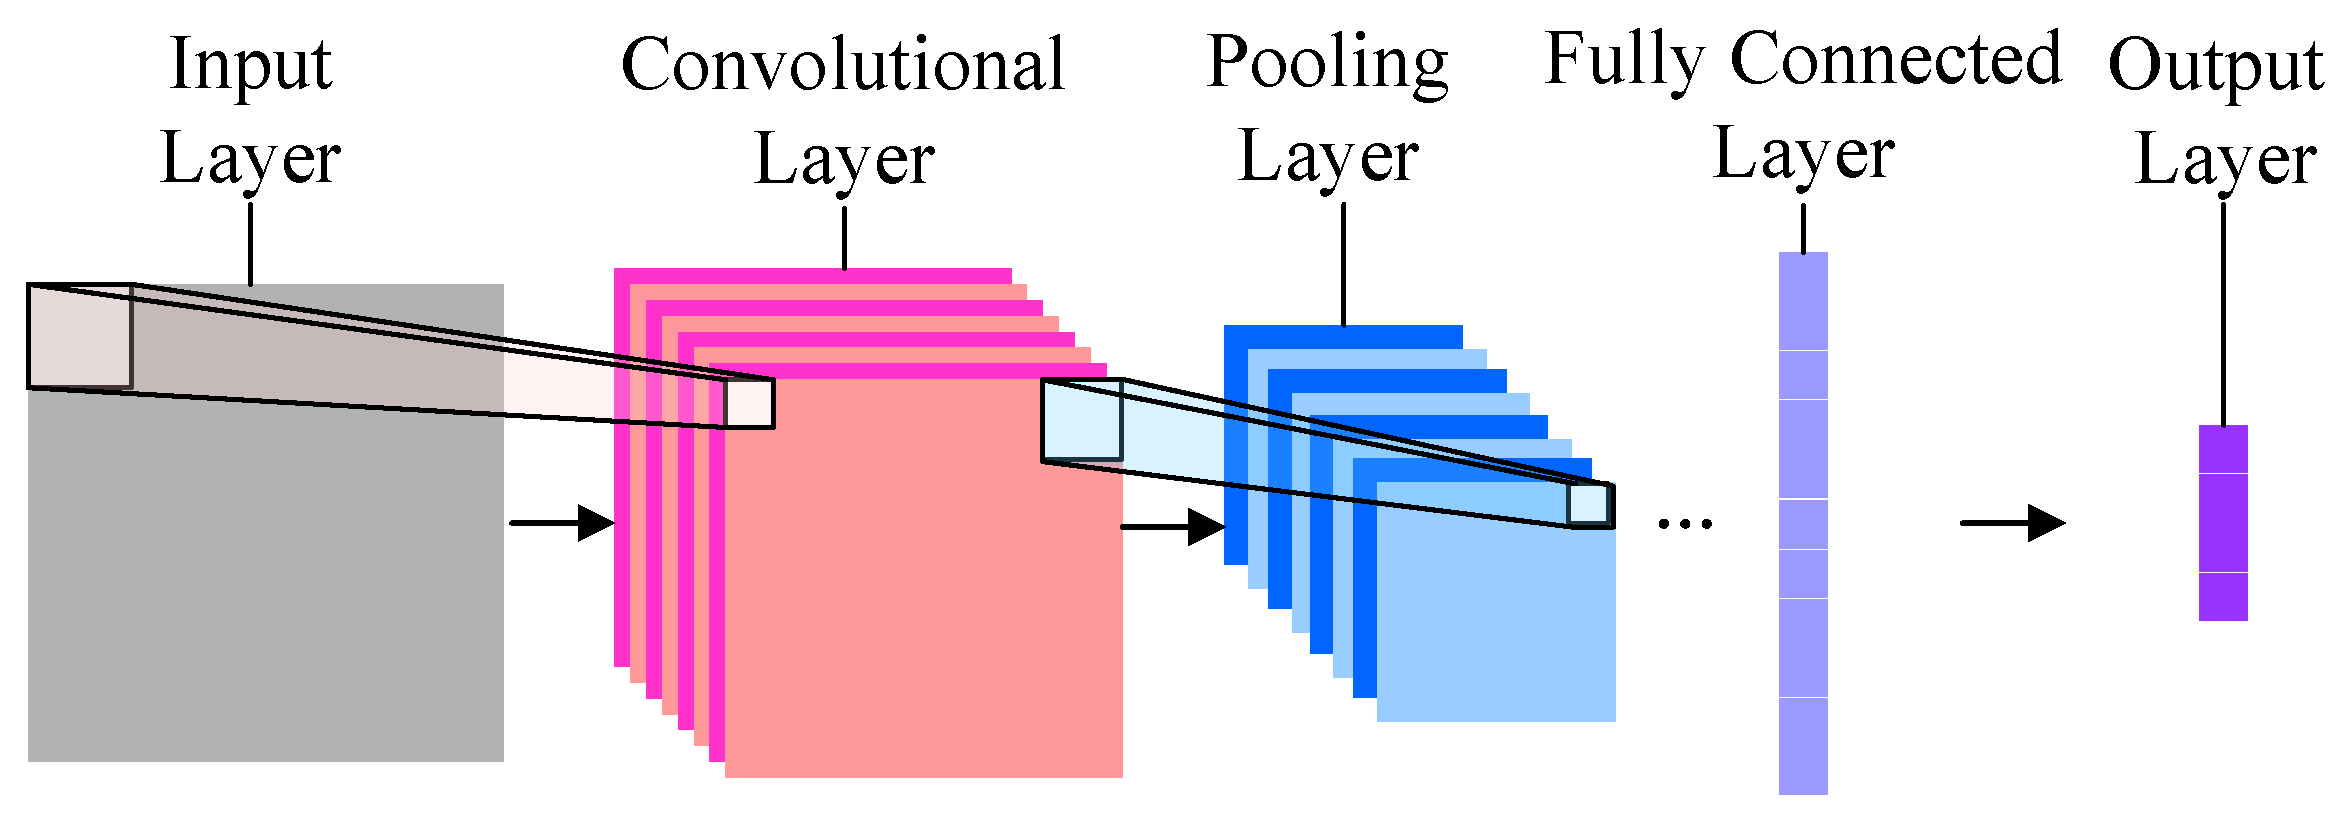
\includegraphics[scale=1]{Figures/CNN3.png}
\caption{卷积神经网络结构}
\end{figure}

卷积神经网络在传统的全连接神经网络结构之外,还引入了以下的结构:
\begin{enumerate}
	
	\item 输入层 INPUT : 预处理多维输入,具有将将输入数据去均值和归一化,再在各个维度上降维形成若干不相关的特征轴功能的神经元层
	\item 激活层 RELU : 应用激励函数的非线性层,具有对线性映射性能不足进行补充,并使输出控制在一定范围内的功能,作为卷积层和输出层的一部分
	\item 卷积层 CONV : 一种基于在特定感受域下的局部感知效应的复杂神经元层
	\item 池化层 POOL : 具有在不同深度上欠采样,降低特征的维度,防止过拟合的功能
	\item 输出层 OUTPUT : 神经网络的最后一层,由线性层和具有概率分布映射功能的$softmax$函数组成,视为多分类器
\end{enumerate}

在不同的层中,多重的卷积层能够更加充分的利用输入的多维特征,而池化层的欠采样功能则能够抛弃多余的特征一在一定程度上避免过拟合的情况.而总体上来说,由于卷积神经网络存在模型参数共用和多维特征采集的机制,导致实际上模型的参数量更精简,实际使用中实用性更高.

\section{卷积神经网络与图像识别}
%来自
%https://zhuanlan.zhihu.com/p/47184529?msclkid=506087dbb97811ec8040aa32dc937a8c

神经网络在图像识别领域的应用是推动整个神经研究领域进步的现实动力之一, 而目前人工神经网络图像识别也成为衡量神经网络性能的重要指标之一.在诸多的人工神经网络模型概念中,卷积神经网络是最有应用价值和研究价值的领域之一.卷积神经元相比全连接的人工神经网络,更加具有广泛应用的潜力.

卷积神经网络相对于全连接的神经网络,能够有效避免全连接网络对多维输入向量化造成的信息损失,同时也避免了全连接网络中大量的冗余参数造成训练困难和过拟合现象.因此,卷积神经网络也在图像识别领域更加具有竞争力和实用性.


下图即是类LeNet卷积神经网络在MNIST手写数据集上的应用.

\begin{figure}
	\centering
	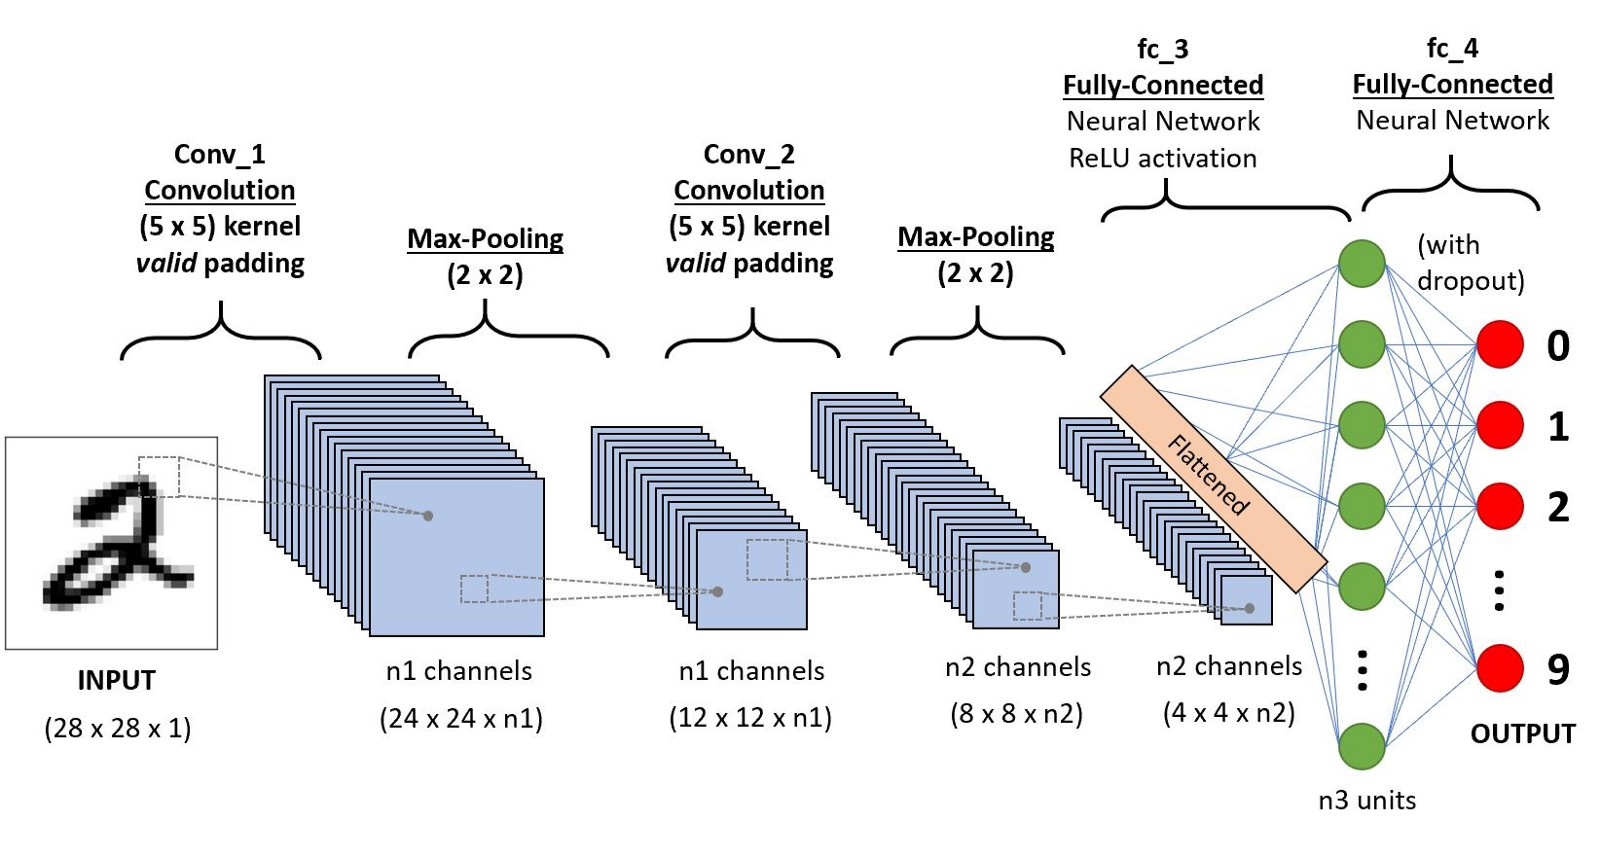
\includegraphics[scale=0.3]{Figures/CNN2.jpg}
	\caption{卷积神经网络在图像识别上的应用}
\end{figure}

\section{本文的目的}

本文意图通过在不同数据下进行差异化训练的同质的卷积神经网络模型在测试集中对特定对象进行"投票式"的预测,并通过比较不同模型间的预测差异,来从目标测试集中选取特定的对象列为疑似的恶意样本.

\chapter{卷积神经网络的投票式模型分析}

\section{MNIST数据集的使用}

MNIST数据集作为在卷积神经网络中被广泛使用的数据集

\section{卷积神经网络的选取}

本次实验选取的是在图像识别领域常用的 LeNet 卷积网络模型